\documentclass{report}

% set font encoding for PDFLaTeX, XeLaTeX, or LuaTeX
\usepackage{ifxetex,ifluatex}

\if\ifxetex T\else\ifluatex T\else F\fi\fi T%
  \usepackage{fontspec}
\else
  \usepackage[T1]{fontenc}
  \usepackage[utf8]{inputenc}
  \usepackage{lmodern}
\fi

\usepackage[margin=0.5in]{geometry}

\usepackage{amsmath}
\usepackage{amssymb}
\usepackage{amsthm}
\usepackage{bm}
\usepackage{bbm}
\usepackage{mathtools}
\usepackage{physics}

\usepackage{enumitem}
\usepackage{multicol}
\usepackage{graphicx}
\usepackage[dvipsnames]{xcolor}

\usepackage{hyperref}
\hypersetup{colorlinks=true,}

\usepackage[parfill]{parskip}
\usepackage{lipsum}
\usepackage[export]{adjustbox}
\usepackage{listings}

\usepackage{xparse} 
\usepackage{subfig} 
\usepackage{xparse} 
\usepackage{float}

\usepackage[sorting=none]{biblatex} 

%%%%%This is an image table command, can likely be deleted
\newcommand{\subf}[2]{

%
{\small 
\begin{tabular}
  [t]{@{}c@{}} #1\ 
  \#2 
\end{tabular}
}

%
} 

\makeatletter
\renewcommand*\env@matrix[1][c]{\hskip -\arraycolsep
  \let\@ifnextchar\new@ifnextchar
  \array{*\c@MaxMatrixCols #1}}
\makeatother
%%%%%% Tensor Product
\NewDocumentCommand{\tens}{e{_^}}{ 
\mathbin{\mathop{\otimes}\displaylimits \IfValueT{#1}{_{#1}} \IfValueT{#2}{^{#2}} }}
%%%%%% Add \R Reals
\newcommand{\R}{\mathbb{R}} 
\newcommand{\N}{\mathbb{N}} 
\newcommand{\Z}{\mathbb{Z}} 
%%%%%% Missing citation warn
\newcommand{\CITEMISSING}{\colorbox{BurntOrange}{CITE ME}}
%%%%%% Add \theorem float
\newtheorem{theorem}{Theorem}
%%%%%% Add \definition float
\theoremstyle{definition} 
\newtheorem{definition}{Definition}[section]
%%%%%%%%%%%%%%%%%%%%%%%%%%%%%%%%%%%%%%%%%%%%%%%%%%%%%%%%%%%%%%%%%%%%%%%%%%%%%%%%%%%%%%%%%%%%%%%%%%%%%%%%%%%%%%%%%%%%%%%%%%
%%%%%Uncomment to add citation library 
\bibliography{lib}
\title{Model Description}
\author{David Helekal}

\begin{document}
\chapter{Model}
\section{Coalescent with Local Population Structure}
We now present novel local phylodynamic model.
In order to help illustrate the concepts behind this model, consider the following scenario:
Suppose there is a parent population of bacteria of interest evolving through time. At any point in time, a particular individual within this population gains a significant evolutionary advantage. This advantage enables the individual and its progeny to undergo a rapid clonal expansion as it gains the ability to colonise a particular niche, eventually reaching a constant population size equilibrium. We will associate the clade corresponding to the clonal expansion with a particular colouring. 
The clonal expansion process may repeat throughout time, giving rise to several clades. The clonal expansions may for example correspond to process such a bacterial strain gaining antibiotic resistance, or being newly introduced into a hospital.

In general, we will assume that the clonal expansion process happens relatively rarely. We will also assume the parent population is at eqillibrium. As under this scenario populations reach a constant population size in the limit this assumption can be interpreted that the clonal expansion that gave rise to the parent population has happened a very long time ago.

At present a researcher collects a random set of $N$ samples from the population of interest, containing at least some of the clades produced by the clonal expansion process described above. Each sample belongs to one of the $k$ clonal expansion clades with probability $\theta_i$, $\pmb{\theta} = [\theta_1, ..., \theta_i, ..., \theta_{k-1}, \theta_{k}]$.

The researcher then sequences the genomes of the samples and infers the corresponding phylogenetic using any of the popular available methods.
The resulting phylogeny can be viewed as a realisation of the following backwards time process. 

Select $M$ clade colours, and an associated clade sampling membership probability vector $\pmb{\theta}$. For each of the $N$ samples $s_i$ forming the leaves of the phylogeny, assign a colouring $c_i$. The samples of identical colour then coalesce with each other with rate governed by a colour specific population size function $\alpha_i(t)$. As it is assumed each colour is formed by a clonal expansion at time $t_{div_i}$, $\alpha_i(t)$ vanishes to zero at the time of the expansion, and as such all coalescence within clade of colour $c_i$ happens almost surely before $t_{div_i}$. Upon reaching the time of clonal expansion the MRCA then chnages colour to that of another clade extant at the time. The clade of the colour the MRCA changes tof will be referred to as the parent clade. The MRCA is then added to the parent clade as a leaf. 
The process continues until all only one individual remains.

The coalescent process given leaf colouring and growth function parameters described above is characterised mathematically in the following section.
%%%%%%%%%%%%%%%%%%%%%%%%%%%%%%%%%%%%%%%%%%%%%%%%%%%%%%%%%%%%
%%%%%%%%%%%%%%%%%%%%%%%%%%%%%%%%%%%%%%%%%%%%%%%%%%%%%%%%%%%%
%%%%%%%%%%%%%%%%%%%%%%%%%%%%%%%%%%%%%%%%%%%%%%%%%%%%%%%%%%%%
%%%%%%%%%%%%%%%%%%%%%%%%%%%%%%%%%%%%%%%%%%%%%%%%%%%%%%%%%%%%
\section{Model}
\subsection{Preliminaries}
A given genealogy $\mathbf{g}=(V_\mathbf{g}, E_\mathbf{g}, t_\mathbf{g}, c_\mathbf{g})$ is an incomplete, empirical sample of the underlying process.\\
It consists of nodes $V_\mathbf{g}$, directed edges $E_\mathbf{g}$, node labels $t_\mathbf{g}$ corresponding to event times, and node labels $c_\mathbf{g}$ corresponding to node colouring.\\
The genealogy $\mathbf{g}$ shall be indexed by an index set $S=1\leq i \leq N\subset \N$, with $Y\subset S$ corresponding to coalescent events and $I\subset S$ corresponding to sampling events.\\
For convenience, assume that all edges are in the forwards time direction, i.e.: 
\begin{gather*}
\forall k,l \in S: (k,l)\in E_\mathbf{g} \Rightarrow t_k>t_l
\end{gather*}
Furthermore, all event times are ordered in descending (backwards) time order, with the first event corresponding the the most recent sample
\begin{gather*}
\forall k,l \in S: k<l \Rightarrow t_k < t_l
\end{gather*}
Under the assumption that $\mathbf{g}$ is a genealogy of a given sample, with each edge in $E_\mathbf{g}$ there is an associated unobserved set of individuals descending from one another. At some point along an edge from one lineage to another, the lineage can undergo a colour change, and become the most recent ancestor of a diverging clade. This event corresponds to this lineage somehow gaining advantage over other lineages, be it a bacterium gaining resistance against a drug, or a strain of a virus invading a completely susceptible population.

\begin{definition}[Multiple Lineage Coalescent]\label{def:model}
Given $M$ colours, $M$ population size functions $\mathbf{\alpha}\triangleq\{\alpha_j(t)\}_{1\leq j\leq M}$, the set of $M-1$ divergence times $T_{div} \triangleq \{t_{div_j}\}_{1\leq j<M}$, the set of $M-1$ divergence events $D \triangleq \{d_j\}_{1\leq j<M}$, the set of tips $I\subset \N, \quad I=\{1,2,...,N\}$, and the associated sampling times $T_{sam}\triangleq \left\{t^s_i\right\}_{i \in I}$.
Assume that the indexing is such that the divergence times are in ascending order.\\
Let $\pmb\Pi(t)$ be a continuous time markov chain defined on the state space of the partitions of $I$ denoted by $\Pi$, each associated with a colouring via the function $H: \Pi\cross\R^+ \mapsto \{1,...M\}$. The initial state is given by $\pmb\Pi(0) = \{1\}, \{2\}, ... , \{N-1\}, \{N\}$.

Denote the number of extant partitions of given colour $j$ at time $t$ by $|C_j(t)| \triangleq |\{\pi \in \Pi(t) : H(\pi, t) = j \}|$

And transition rates
\begin{gather}\label{eq:transitions}
q_{(\pi_i,\pi_j), (\pi_i\cup\pi_j)}=\lim\limits_{h \downarrow 0}\frac{1}{h}\mathbf{P}\left[\pi_i \cup \pi_j \in \pmb\Pi(t+h)\mid \pi_i, \pi_j \in \pmb\Pi(t), \pi_i \neq \pi_j \right]  
\end{gather}
given by
\begin{gather}\label{eq:rates}
q_{(\pi_i,\pi_j), (\pi_i\cup\pi_j)} = \sum\limits_{k=1}^{M} \delta_k(H(\pi_i,t))\delta_k(H(\pi_j,t))\frac{\binom{C_k(t)}{2}}{\alpha_k(t)}
\end{gather}
\end{definition}
Finally, $H$ is defined recursively with $\forall \pi_i \in \pmb\Pi(0), H(\pi_i,0) = c_{i,0}$ with $c_{i,0}$ given. For fixed $t$ and and $\forall \pi \in \pmb\Pi(t)$, The colouring function satisfies $H(\pi, t) = H(\pi_0,t)\quad \forall \pi_0 \in \pmb\Pi(0) : \pi_0 \subset \pi$. In time, $H$ is defined so that $\forall \pi \in \pmb\Pi(0) : H(\pi,0) = j,\quad \forall t>0 \quad H(\pi, t) = \begin{cases} 
      j & t < T_{div_j} \\
      d_j & t \geq T_{div_j}
   \end{cases}$\\
   
While the model is defined in terms of partitions, when working with genealogies we typically work with trees. The tree corresponding to a particular realisation of the partition based model is obtained by identifying all $\pi \in \pmb\Pi(t)\forall t$ with $V_\mathbf{g}$. The leaves $V_I$ consist of all partitions $\pi \in \pmb\pi(0)$, while internal nodes $V_Y$ consist of all subsequent partitions $\forall t, \forall\pi\in \pmb\Pi(t) : \pi \notin \pmb\Pi(0)$. The edges $V_\mathbf{g}$ and times $t_\mathbf{g}$ are given by the jump chain. The colouring $c_\mathbf{g}$ is obtained through the colouring function $H$. 

The interpretation of this model in backwards (coalescent) time is that each node corresponds to a single specific clade (colour). Nodes of the same clade coalesce at i.i.d rates, according to a clade specific growth functions, until reaching the most recent common ancestor (MRCA) of given clade. The MRCA then changes type (colour) to that given by the corresponding divergence event at corresponding divergence time time. 

Within-colour transitions and their rates are independent of different colours. As such the transitions involving partitions of one colour  are independent of transitions involving partitions of other colours given divergence events and times. This allows us to split the likelihood computation into a product of colour-specific likelihoods, that can be computed under coalescent with variable population size.\\
\subsection{Likelihood Under Multiple Lineage Coalescent}
%%%%%%%%%%%%%%%%%%%%%%%%%%%%%%%%%%%%%%%%%%%%%%%%%%%%%%%%%%%%
%%%%%%%%%%%%%%%%%%%%%%%%%%%%%%%%%%%%%%%%%%%%%%%%%%%%%%%%%%%%
%%%%%%%%%%%%%%%%%%%%%%%%%%%%%%%%%%%%%%%%%%%%%%%%%%%%%%%%%%%%
%%%%%%%%%%%%%%%%%%%%%%%%%%%%%%%%%%%%%%%%%%%%%%%%%%%%%%%%%%%%
\section{Full Model}
Given a population sample of $N$ individuals indexed by $F$, $X_F = \{x_i\}_{i \in F}$, first determine the number of recent clonal expansions $M-1$:
\begin{gather}
M-1 \sim \texttt{poi}(\phi)
\end{gather}
Then simulate the $M$-dimensional clonal expansion probability vector $\pmb{\theta}$:
\begin{gather}
\pmb{\theta} \sim \texttt{dirichlet}(\psi), \quad \psi \in \R_+^{M} 
\end{gather}
Given the number of expansions $M-1$ and expansion probabilities $\pmb{\theta}$, partition $F$ into $M$ mutually disjoint subsets $\mathbf{f}=\{f_1, ... f_{M-1}, f_{M}\}$ with $\bigcup\limits_{i=1}^{M} f_{i} = F$ with the probability $P[j\in f_{i}]=\theta_i\quad \forall i,\forall j \in F$.  
Each partition corresponds to an individual colour characterising a clonal expansion. For convenience, we will set $f_{M}$ to be the index set of the tips corresponding to the parent subpopulation.

The sample along with the initial colour assignment then follows the coalescent process described above in \ref{def:model}, governed by population size functions $\alpha_{j}(t)$. To each $\alpha_{j}$ corresponds a set of parameters:
\begin{gather}
\begin{aligned}
t_{div_{j}}\in\R_+ \quad&\text{The time of divergence}\\
r_j\in\R_+\quad&\text{The growth rate of the subpopulation}\\
N_j\in\R_+\quad&\text{The carrying capacity}
\end{aligned}
\end{gather}
The divergence events $d_i$ are simulated so that an expansion with divergence time $t_{div_j}$ merges with and thus changes colour to that of an expansion chosen uniformly at random from all expansions with time of divergence after $t_{div_j}$, i.e. an expansion that is extant at time $t_{div_j}$.

In the case of the parent subpopulation $f_{M}$, we assume that the divergence event happened a very long time ago. As by definition $\alpha(t) \rightarrow N$ as $t_{div}-t\rightarrow \infty$, we approximate $\alpha_{M}(t) \approx N_{M}$ and as such $\alpha^{-1}_{M}(t) \approx 1/N_{M}$. The parameters $t_{div_{j}}, r_j, N_j$ are simulated from appropriate (prior) distributions.
Finally, without loss of generality, assume that divergence events are indexed in ascending order by the time of divergence in coalescent time.
\begin{gather}
i > j \Leftrightarrow t_{div_i} > t_{div_j}  
\end{gather}
Sampling times $\mathbf{t}=\{t_i\}_{i\in F}$ are simulated from the same distribution for all $f$. It is required that for all expansions $j$, $t_i < t_{div_j}$, for all $i \in f_j$. In other words, all sampling for a given clade must happen before the clade diverges. As such we assign zero likelihood if any sampling occurs after clade divergence.
\subsubsection{Choice of effective population size functions}
While the parent clade is assumed to be at equilibrium, the population size functions of the diverging clades have to satisfy several properties.\\
First we introduce the variable $\tau = -t + t_{div}$ which denotes time relative to a divergence event of a given clade, where $t_{div}$ denotes the divergence time.
In our model we assume that the diverging subpopulation only appears after the divergence event, and as such it is required that at time $\tau=0$ the population vanishes $\alpha(\tau)=0$. Furthermore, we are looking for a monotone increasing function in $\tau$, that exhibits saturating behaviour as $\tau$ grows large.
Initially, functions exhibiting a period of exponential growth were investigated, however these were ill-posed numerically.
Hence we arrived at the following function
\begin{gather}
\alpha(\tau) = N\frac{r\tau^2}{1+r\tau^2}
\end{gather} 
Where $N$ is the carrying capacity and $r$ is the growth rate.
This function  exhibits saturating behaviour.\\
While the intepretation of the carrying capacity $N$ is straightforward, we find $r$ to be best intepreted by considering the time to when the population reaches half the carrying capacity $t_{mid}$ as a function of $r$. It is straightforward to show that $t_{mid}(r) = \frac{1}{\sqrt{r}}$ 
\begin{figure}[H].
  \centering
     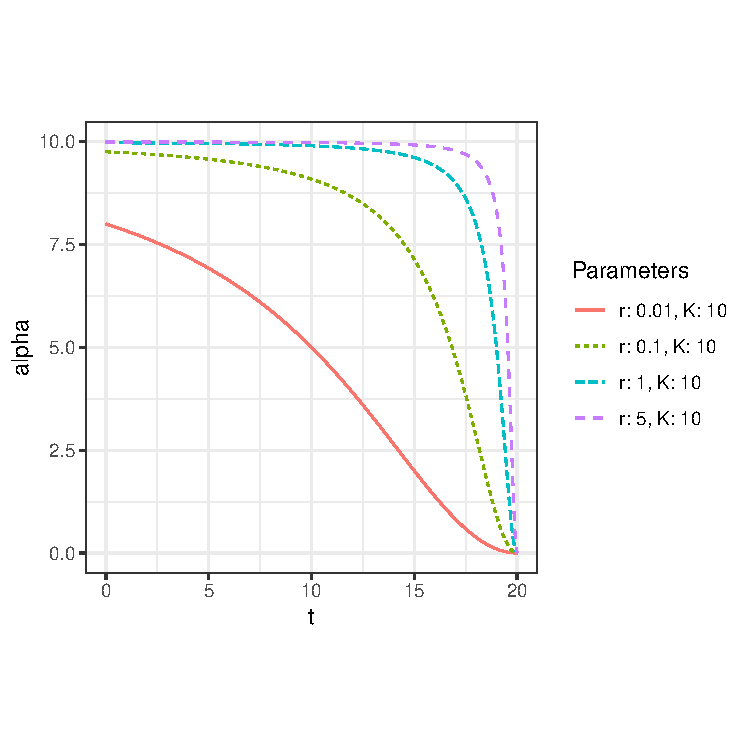
\includegraphics[width=0.4\textwidth]{../R/test_mcmc/alpha_plots}
    \caption{$\alpha(\tau)$ under different parameters, with $T_{div}=20$}
\end{figure}
The integral of the reciprocal $\alpha^{-1}(\tau)$ under this formulation is then given by 
\begin{gather}
\begin{aligned}\label{eq:rint}
&\int_{t}^{t+s}\alpha^{-1}(\tau)\,d\tau\\ &= \frac{1}{N}\left[-\frac{1}{r(-\tau+t_{div})}-\tau+t_{div}\right]_{t}^{t+s}
\end{aligned}
\end{gather}
As $t+s$ approaches the divergence time relative to the most recent sample $T_{div}$, the rate integral \ref{eq:rint} approaches infinity, and as such all coalescence within a clade happens before time of divergence with probability one.

For the purposes of our model, we simulate the parameters $N_j, r_j, t_{div_j} \forall j \in \{1,...,M-1\}$ as well as the parent population size $N_{M}$ under the following scheme.\\
First simulate the parent population size $N_{M}$:
\begin{gather}
N_{M} \sim \texttt{lognorm}(\mu_{anc}, \sigma_{anc})
\end{gather}
Next simulate the carrying capacities for the $M-1$ expansions
\begin{gather}
N_{j} \sim \texttt{lognorm}(N_{M}, \sigma_{exp}) \quad\forall j \in \{1,...,M-1\}
\end{gather}
as well as the corresponding divergence times
\begin{gather}
t_{div_j} \sim \texttt{gamma}\left(\frac{\nu^2}{\kappa^2}, \frac{\kappa^2 N_M}{\nu}\right) \quad\forall j \in \{1,...,M-1\}
\end{gather}
where $\beta \in (0,1)$.
Rather than simulating the growth rates directly, we simulate the correspondng time to midpoint $t_{mid}(r_j) = 1/\sqrt{r_j}$
\begin{gather}
t_{mid}(r_j) \sim \texttt{exp}(\lambda_r/N_M) \quad\forall j \in \{1,...,M-1\}
\end{gather} 
\subsubsection{Summary}
We now summarise the entire simulation procedure
\begin{gather}
\begin{aligned}
&\pi(M-1) &=& \texttt{poi}(\phi) &\quad&\text{Number of expansions} \\
&\pi(\pmb\theta\mid M) &=& \texttt{dirichlet}(\psi) &\quad&\text{Expansion Membership Probabilities} \\
&\pi(\mathbf{f\mid\pmb\theta}) &=& \prod\limits_{j=1}^M\theta_j^{|f_j|}&\quad&\text{Expansion Membership Assignment} \\
&\pi(N_M) &=& \texttt{lognorm}(\mu_{anc},\sigma_{anc}) &\quad&\text{Parent Population Size}\\
&\pi(N_j\mid N_{M}) &=& \texttt{lognorm}(N_{M},\sigma_{exp})\quad\forall j \in \{1...M-1\} &\quad&\text{Carrying Capacities}\\
&\pi(d_j\mid T_{div}, M) &=& U(\{i\in \{1 ... M+1\} : t_{div_i} > t_{div_j}\}) &\quad&\text{Parent Populations}\\
&\pi(t_{div_j}\mid N_{M}) &=& \texttt{gamma}\left(\frac{\nu^2}{\kappa^2}, \frac{\kappa^2 N_M}{\nu}\right) \quad\forall j \in \{1...M-1\} &\quad&\text{Expansion Times}\\
&\pi(t_{mid}(r_j)\mid N_M) &=& \texttt{exp}(\lambda_{r}/N_M)\quad\forall j \in \{1...M-1\} &\quad&\text{Growth Rates/Time to Midpoint}
\end{aligned}
\end{gather}

Note that the expansion parameters are exchangeable.

For convenience, we will summarise $\pi(N_M)\prod\limits_{j=1}^{M-1}\pi(N_j\mid N_{M})\pi(t_{div_j}\mid N_{M})\pi(t_{mid}(r_j)\mid N_M)$ as $\pi(\pmb\alpha)$.

The tip times $T_{sam}$ are simulated separately and considered given. Furthermore $T_{sam} \perp M, \mathbf{f}, \pmb{\theta}, \pmb\alpha, D, T_{div}$.

The genealogy $\mathbf{g}$ is simulated under the Coalescent with Local Population structure described in \ref{def:model} denoted by $\texttt{lpcoal}$:
\begin{gather}
\pi(\mathbf{g}\mid M, \mathbf{f}, \pmb\alpha, T_{div}, D, T_{sam}) = \texttt{lpcoal}(M, \mathbf{f}, \pmb\alpha, T_{div}, D, T_{sam})
\end{gather} 

$\phi, \psi, \mu_{anc}, \sigma_{anc}, \mu_r, \sigma_r, \sigma_{exp}, \nu, \kappa$ are hyperamaters and considered given. The mean of divergence times $\mathop{\mathbb{E}}[T_{div}]$ is equal to $\nu N_m$ and the standard deviation of $t_{div}$ is $\kappa N_M$.


%%%%%%%%%%%%%%%%%%%%%%%%%%%%%%%%%%%%%%%%%%%%%%%%%%%%%%%%%%%%
%%%%%%%%%%%%%%%%%%%%%%%%%%%%%%%%%%%%%%%%%%%%%%%%%%%%%%%%%%%%
%%%%%%%%%%%%%%%%%%%%%%%%%%%%%%%%%%%%%%%%%%%%%%%%%%%%%%%%%%%%
%%%%%%%%%%%%%%%%%%%%%%%%%%%%%%%%%%%%%%%%%%%%%%%%%%%%%%%%%%%%
\subsection{Posterior}
The posterior for the full process is:
\begin{gather}
\begin{aligned}
P(M-1, \mathbf{f}, \pmb{\theta}, \pmb{T_{div}}, \mathbf{r}, \mathbf{N}\mid\mathbf{g})
&\propto \pi(\mathbf{g}\mid M, \mathbf{f}, \pmb\alpha, D)\\
&\cross \pi(\pmb\alpha\mid M)\\
&\cross \pi(D\mid \pmb\alpha,M)\\
&\cross \pi(\mathbf{f}\mid\pmb{\theta}, M)\\
&\cross\pi(\pmb{\theta}\mid M)\pi(M)\\
&\cross (M-1)!
\end{aligned}
\end{gather}
The final $(M-1)!$ term is due to expansions being exchangeable.
\section{RjMCMC Moves}
For inference we use reversible jump MCMC in order to explore the space of models with varying number of clonal expansions.
The MCMC moves consist of five within model moves, as well as one transdimensional move that adds or removes clonal expansions.\\
We will be using the structure of the tree to guide our proposal distributions. It is worth noting that divergence of a lineage effectively occurs along a branch. We can justify this by noting that a given tip partition corresponding to a certain colour must fully coalesce with itself up to the MRCA of the lineage before changing colour to that of its parent. This is because the effective population size vanishes as the divergence time reached.
The branch along which the lineage divergence occurs is the one leading into the lineage MRCA. It remains to demonstrate that the the divergence time for a lineage cannot exceed the time of parent of this branch. This is straightforward as the divergence time being greater than the parent of the branch leading into the lineage MRCA would imply that partitions with different colouring coalesced - an event that happens with probability zero.\\
In order to efficiently explore all tip partitions compatible with the genealogy given, tip partitions are generated by selecting a branch along which a divergence of a a given colour is supposed to happen. All tips corresponding to the clade that has the child node along the branch as its MRCA are then assigned to the given colour, with the exception of tips that correspond to clades that diverge earlier. 
\subsection{Within Model Moves}
We will use the following notation to describe updates.\\ Let 
\begin{gather}
x^{(M)}_{r_j\to r^{'}}
\end{gather}
Denote the update of rate parameter $r_j$ corresponding to the $j$-th clonal expansions to the value $r^{'}$ in the $M$-expansion model. Analogously, all within model updates will be denoted this way.\\

The within model updates will now be described.\\
The first move is:
\begin{gather}
x^{(M)}_{\left(t_{mid_j},N_j\right)\to \left(t_{mid}^{'},N^{'}\right)}\quad\forall j < M
\end{gather}
This move updates simultaneously the growth rate and the carrying capacity of the expansion. The new values are distributed according to
\begin{gather}
\left(t_{mid}^{'},N^{'}\right)\sim\left(\mathcal{N}(t_{mid_j}, \sigma_r), \texttt{lognorm}(log(N_j), \sigma_K)\right) 
\end{gather}\\
The proposal ratio of this move is:
\begin{gather}
\frac{f_{ln}(N_j;log(N^{'}), \sigma_K)}{f_{ln}(N^{'};log(N_j), \sigma_K)}
\end{gather}
Where $f_{ln}(x; a, b)$ stands for the value of the lognormal distribution pdf with log-mean $a$ and log-standard deviation $b$ evaluated at $x$.

The second move is:
\begin{gather}
x^{(M)}_{t_{div_j}\to t_{div}^{'}}\quad\forall j < M
\end{gather} 
This move updates the divergence time of the $j$-th expansion. The new values are distributed according to
\begin{gather}
t_{div}^{'}\sim\mathcal{N}(t_{div_j}, \sigma_t)
\end{gather}
$\sigma_t$ is chosen dynamically as a fixed fraction of the length of the branch that corresponds to this divergence event. This is the branch that leads into the MRCA of this clonal expansion.\\
The proposal ratio of this move is $1$.

The third move is:
\begin{gather}
x^{(M)}_{\left(\mathbf{f}, t_{div_j}, D\right)\to \left(\mathbf{f}^{'}, t_{div}^{'}, D^{'}\right)}
\end{gather} 
This moves updates the colouring of the leaves and thus the memberships of clonal expansions. This is perhaps the most complicated move and proceeds as follows: \\
Let $b_j$ denote the branch along which the divergence event for the $j$-th expansion lies, i.e. the branch leading into the MRCA of the expansion, and with $m_j$ the MRCA of the expansion. Let $\beta_1$ be a bernoulli variable with probability $1/2$. decide which direction to update the MRCA in. If $\beta_1=0$ move upwards in the tree. In this case there is only one eligible branch as in a tree the MRCA node only has one parent. If $\beta_1 = 1$ move downwards, with probability $1/2$ select one of the branches that lead into the child nodes of the MRCA. Denote the new branch as $b^{'}$, and the new MRCA, that is the child node along branch $b^{'}$, as $m^{'}$.
We update time so that it is compatible with the new tip partition. The updated time by $t_{div}^{'}$ is distributed according to
\begin{gather}
t_{div}^{'}\sim U((t_{b^{'}_2}, t_{b^{'}_1}))
\end{gather}
where $t_{b^{'}_1}$ and $t_{b^{'}_2}$ are the times of the child and parent nodes of the branch $b^{'}$ respectively. 
Colour the tips corresponding to the clade defined by $m^{'}$, with the exception of tips corresponding to clades that diverge earlier as described previously in this section.
Finally, set the parent populations $D^{'}$ so that they are compatible with the updated divergence times and tip partition. This is done for each expansion $i$, by setting $d_i$ to be equal to the lineage membership of the parent node of the MRCA of expansion $i$.\\
The proposal ratio for this move is:
\begin{gather}
\frac{\left(t_{b^{'}_1}-t_{b^{'}_2}\right)\left(1-\frac{1}{2}\delta_0\left(\beta_1\right)\right)}{\left(t_{b_{j_1}} - t_{b_{j_2}}\right)\left(1-\frac{1}{2}\delta_1\left(\beta_1\right)\right)}
\end{gather}

The fourth move updates the probabilities vector $\pmb \theta$:
\begin{gather}
  x^{(M)}_{\pmb\theta\to \pmb\theta^{'}}
\end{gather}
For this move first simulate indices $k, l\sim U(\{1...M\})$. Next simulate $u\sim U((0, \theta_k))$. Set $\theta^{'}_i = \theta_i \quad\forall i \in \{1...M\}\setminus\{k,l\}$ and $\theta^{'}_k = \theta_k-u$, $\theta^{'}_l = \theta_l+u$.\\
The proposal ration for this move is:
\begin{gather}
\frac{\theta_k}{\theta^{'}_l}
\end{gather}

The fifth and final move updates the effective population size $N_M$ of the parent population:
\begin{gather}
x^{(M)}_{N_M\to N^{'}}
\end{gather}
With distributed according to
\begin{gather}
N^{'}\sim \mathcal{N}(N_M, \sigma_N)
\end{gather}
The proposal ration for this move is $1$.
\subsection{Transdimensional moves}
The move that removes an expansion $x^{(M)\to(M-1)}$ proceeds by selecting an expansion index $k$ uniformly at random from $\{1...M-1\}$ ($M-1$ as parent population cannot be removed), removing the associated parameters from the parameter vector and setting $M^{'} = M-1$. The tip partition $\mathbf{f}$ is updated by colouring tips according to the scheme mentioned in the previous section using the new parameter vector with the $k$-th expansion parameters removed. The probability vector $\pmb\theta^{'}$ is updated by first selecting $l$ uniformly at random from $\{1...M^{'}\}$, and setting $\theta^{'}_i = \theta_i\quad \forall i:i<k,i\neq l$, $\theta^{'}_i = \theta_{i+1}\quad \forall i:i\geq k,i\neq l$ and finally $\theta^{'}_l = 
  \begin{cases} 
      \theta_l+\theta_k & l < k \\
      \theta_{l+1}+\theta_k & l \geq k
  \end{cases}$.\\
The proposal ratio for this move is:
\begin{gather}
\frac{(M-1)\cross(M-1)\cross\pi(N^{'}\mid N_{M})\cross\pi(t^{'}_{div}\mid N_{M})\cross\pi(r^{'})}{\theta^{'}_l\cross(M-1)}
\end{gather}

The reverse move that adds an expansion $x^{(M)\to(M+1)}$ 
proceeds by setting $M^{'} = M+1$ and simulating expansion parameters from the priors as:
\begin{gather}
\begin{aligned}
N^{'} &\sim \pi(N\mid N_{M})\\
t^{'}_{div} &\sim \pi(t_{div}\mid N_{M})\\
r^{'} &\sim \pi(r)
\end{aligned}
\end{gather}
The new expansion is added under the index $M^{'}-1$. The tip partition $\mathbf{f}$ is updated by adding a new colouring, such that it is not identical to an existing colouring, and so that the clade defined by this colouring coalesces with itself before $t_{div^{'}}$. Furthermore the parent clade $d^{'}$ must be selected so that the MRCA of the diverging clade coalesces with a node of the parent clade after $t_{div^{'}}$. This can be done by first selecting a branch $b'$ uniformly at random from all branches with child node before $t_{div^{'}}$ and parent node after $t_{div^{'}}$. Next, setting the new partition to be all leaves belonging to the clade with the MRCA given by the child node of $b'$ excluding those that belong to diverging clades with time of divergence before $t_{div^{'}}$. Finally, the parent population vector $D^{'}$ has to be updates by for expansion $i$ setting $d_i^{'}$ to be equal to the expansion membership of the parent node of the MRCA of expansion $i$.\\
The probability vector $\pmb\theta^{'}$ is updates by selecting $k$ uniformly at random from $\{1...M\}$, and $u\sim U((0, \theta_k))$. Set 
\begin{gather}
  \theta^{'}_i = 
  \begin{cases} 
      \theta_i & i < M, i \neq k \\
      \theta_i-u& i < M, i = k \\
      u & i = M\\
  \end{cases}
\end{gather}
Then set 
\begin{gather}
  \theta^{'}_{M^{'}} = 
  \begin{cases} 
      \theta_M & k \neq M \\
      \theta_M-u& k=M
  \end{cases}
\end{gather}\\
The proposal ration for this move is:
\begin{gather}
\frac{\theta_k\cross(M)}{(M)\cross(M)\cross\pi(N^{'}\mid N_{M})\cross\pi(t^{'}_{div}\mid N_{M})\cross\pi(r^{'})}
\end{gather}

When selecting a move, we first select whether to do a within model move or a transdimensional move with probability $1/2$.
Next if within model moves are selected, we undertake one of the within model moves with equal probability. If transdimensional moves are selected, we choose whether to increase or decrease the number of expansions with probability $1/2$.
\chapter{References}
\printbibliography
\end{document}